\chapter{Renderização interativa de perfis de difusão}
\label{chap::renderizacao_interativa_de_perfis_de_difusao}

\todo[inline]{Perfis de difusão? Ou ODFs? Vamos evitar uso de termos distintos para referenciar um mesmo objeto?}

%\todo[inline]{Falta contextualizar nos objetivos que você listou na seção 1.3. Não é melhor focar em renderização de perfis de difusão que é um dos problemas relacionados diretamente com a interatividade?}

\textcolor{red}{Embora as ODFs proveem informações mais precisas sobre as direções de potenciais fibras que cruzam um \textit{voxel}, a grande quantidade de dados numéricos envolvidos em ODFs de um volume de ressonância magnética ponderada por difusão torna difícil avaliar a plausibilidade das amostras adquiridas em relação à anatomia da substância branca cerebral e aplicá-las para provas de conceito de esquemas de aquisição de tensores de alta ordem. A forma mais comum de superar esta dificuldade é visualizar os dados numéricos das ODFs em glifos provenientes da superfície definida pela plotagem polar esférica $R(\mathbf{\hat{u}})$. Estes glifos permitem sintetizar numa única imagem não só o comportamento local (intravoxel) de difusão como também as relações intervoxeis.} 

\sout{A forma mais comum de visualizar dados derivados de ODFs é através glifos provenientes da superfície definida pela plotagem polar esférica $R(\mathbf{\hat{u}})$. Esta classe de superfície permite a inferência e inspeção de ODFs de difusão e sua distribuição de fibras subjacentes. Adicionalmente, permite a avaliação visual das ODFs obtidas a partir de um método HARDI para diferentes aquisições. Estes glifos dão uma visualização clara do comportamento local de difusão e são amplamente utilizados para provas de conceito em trabalhos na área de HARDI e essenciais para visualização dos resultados gerados pelos métodos de alta ordem.}

\sout{Alguns dos exemplos de}\textcolor{red}{Entre os} trabalhos que \textcolor{red}{utilizam} os \textcolor{red}{glifos}\sout{utilizam}, temos\sout{:} \citeonline{TuchQBall2004},  \citeonline{yeh2010},  \citeonline{daducci2014}  e  \citeonline{descoteaux2007}. \citeonline{TuchQBall2004},  \citeonline{yeh2010} os utilizam como ferramenta de visualização para o\textcolor{red}{s} método\textcolor{red}{s} de imageamento propostos em seus respectivos trabalhos. \citeonline{daducci2014} os utiliza para ilustrar e comparar ODFs reconstruídas por diferentes métodos. E \citeonline{descoteaux2007} \textcolor{red}{aplicam os glifos}  para ilustrar transformações entre ODFs \todo{Não entendi nos seus respectivos algoritmos de tractografia!}\textcolor{magenta}{nos seus respectivos algoritmos de tractografia propostos}. \todo{Não entendi a observação. GQI foi uma técnica que você escolheu para gerar ODFs ... Em tese, ODFs podem ser geradas por outras técnicas.}\sout{Isto evidencia que o algoritmo de renderização que estamos propondo não é restrito somente ao método GQI que apresentamos no Capítulo \ref{chapter::metodos_hardi}.}
\textcolor{red}{Além de proporcionar melhor entendimento dos dados adquiridos pelas técnicas de alta ordem, conjeturamos que a visualização das ODFs através de glifos posicionados em seus respectivos \textit{voxels} sobrepostos a um volume de ressonância magnética ponderada em T1 pode melhorar o processo de escolha de sementes para tractografias baseadas em sementes. \citeonline{voltoline2021} trazem algumas evidências das circunstâncias em que os superquádricos do DTI podem melhorar este processo.}

\todo[inline]{Sugiro que você expanda o seguinte parágrafo tocando brevemente (1) o foco desta dissertação (visualização interativa de ODFs $\rightarrow$ renderização de ODFs em tempo interativo em GPU); (2) potenciais problemas (tráfego CPU-GPU, limitada memória da GPU, otimização na renderização) $\rightarrow$ mapeamento de ODFs em modelos geométricos, redução de tráfego, ocupação da memória de GPU;  e (3) o estado-da-arte.}

\textcolor{magenta}{
Neste capítulo, apresentamos o algoritmo de renderização interativa de ODFs através de glifos, integrado ao ambiente de visualização multimodal para visualização DWI. Mostraremos como resultados aspectos visuais e sua performance, na qual atestamos a sua interatividade.
}

\textcolor{magenta}{O capítulo está organizado em 5 seções. Na Seção \ref{sec::glifos_odf} descreveremos a superfície e cor dos glifos, no qual chamaremos de glifos ODF; na Seção \ref{sec::trabalhos_relacionados}, apresentamos os trabalhos relacionados; na Seção \ref{sec::superquadricas}, apresentamos brevemente a \textit{pipeline} de renderização multimodal para superquádricos proposto por \citeonline{voltoline2021}; na Seção \ref{sec::renderizacao_de_glifos_ODF}, apresentamos a modificação na \textit{pipeline} da renderização multimodal para superquádricas e a nossa abordagem para renderização de glifos ODF; na Seção \ref{sec::experimentos}, mostramos a performance do esquema de renderização e aspectos visuais.
}
\textcolor{magenta}{
Na Subseção \ref{ssec::aspectos_visuais}, mostramos que esses glifos são mais informativos que os superquádricos por permitir o inferimento do cruzamento de fibras.
}

\sout{Este algoritmo de renderização, integrado a um sistema de visualização para DWI pode ser uma ferramenta poderosa para pesquisadores da área para avaliar perfis de difusão locais e melhorar o seu entendimento em métodos de alta ordem.
Adicionalmente, temos a conjectura que as ODFs representadas através de glifos posicionados em seus respectivos \textit{voxels} no ambiente de visualização multimodal pode melhorar o processo de escolha de parâmetros iniciais em tractografia. \citeonline{voltoline2021} trazem algumas evidências das circunstâncias que os superquádricos do DTI podem melhorar este processo, e conforme mostramos na Subseção \ref{ssec::aspectos_visuais}, mostramos que esses glifos são mais informativos que os superquádricos por permitir o inferimento do cruzamento de fibras.
}

\sout{O capítulo está organizado em 5 seções. Na Seção \ref{sec::glifos_odf} descreveremos a superfície e cor dos glifos, no qual chamaremos de glifos ODF; na Seção \ref{sec::trabalhos_relacionados}, apresentamos os trabalhos relacionados; na Seção \ref{sec::superquadricas}, apresentamos brevemente a \textit{pipeline} de renderização multimodal para superquádricos proposto por \citeonline{voltoline2021}; na Seção \ref{sec::renderizacao_de_glifos_ODF}, apresentamos a modificação na \textit{pipeline} da renderização multimodal para superquádricas e a nossa abordagem para renderização de glifos ODF; na Seção \ref{sec::experimentos}, mostramos a performance do esquema de renderização e aspectos visuais.}


%\todo[inline]{Eu deixaria o parágrafo abaixo para conclusões}

\section{Trabalhos Relacionados}
\label{sec::trabalhos_relacionados}

Apesar da relevância reconhecida da renderização interativa de dados de ODF, a comunidade não tem explorado muito esta questão. \sout{Por questões de performance}\textcolor{red}{Para poder atender ao requisito de interatividade}, \sout{nos limitaremos}\textcolor{red}{limitáremo-nos} a trabalhos que exploram recursos da GPU. Há duas grandes abordagens \sout{achadas na literatura} para renderização de glifos. A primeira é baseada em \textit{ray-casting}, onde a geometria do glifo é representada por uma função ou expressão algébrica \cite{peeters2009, almsick2011}. A outra é baseada na renderização de malhas, com a geometria do glifo aproximada por malhas poligonais \cite{shattuck2008}.

\todo[inline]{Sendo uma dissertação, você deve discutir melhor as técnicas apresentadas em relação à solução dada à lista dos potenciais problemas.}

\citeonline{shattuck2008} tessela uma representação polar de ODF com triângulos, onde a superfície do glifo é gerada através da discretização do seu domínio polar, e sua forma é gerada na CPU através de uma função analítica neste domínio. Os glifos são renderizados por fatia. Com a mudança de malha e parâmetros de visualização, os vertices do glifo são re-computados e reenviados à GPU. A performance relatada é de dez \textit{frames}/s para uma fatia de um volume, no qual cada glifo tem 225 vértices, em uma cena com aproximadamente 2 milhões de triângulos. Neste trabalho, exploramos recursos da GPU modernos para melhorar a performance de renderização e seu uso de memória.


\citeonline{peeters2009} apresentaram um esquema de renderização utilizando \textit{ray-casting}. Na CPU, o centro, o raio da esfera delimitadora e o cubo delimitador por glifo são computados. Na GPU, o algoritmo de ray-casting é executdo por pixel no \textit{fragment shader}. Se o raio lançado para um pixel não intercepta a esfera delimitadora, o fragmento é descartado. Caso contrário, o algoritmo executa uma busca linear ,com passos discretos para interseção da ODF para com o raio. Eles alcançaram uma melhor performance que o algoritmo apresentado por \citeonline{shattuck2008}. \citeonline{almsick2011} melhorou a busca por interseção utilizando o método numérico \textit{regula falsi} e cilindros delimitadores alinhados com o eixo de visão. Eles atingiram um melhor tempo de performance sem sacrificar a qualidade de renderização, documentando que 9000 glifos puderam ser gerados a 30 FPS. Há um problema crítico na acurácia e eficiência do raio lançado. Quando o raio tende a ser paralelo ao glifo, muitas iterações podem ocorrer em algumas \textit{threads}. A renderização baseada em triângulos que propomos neste trabalho não apresenta este problema. 

\citeonline{voltoline2021} propuseram um esquema de renderização para glifos superquádricos para tensores de difusão \cite{Kindlmann2004}. Eles exploraram recursos modernos da GPU para atingir este objetivo, que consistem em \textit{transform feedback}, aproximação triangular adaptativa dos glifos e renderização por instanciação indireta. Diferentemente das superquádricas, os dados associados com glifos ODF tem dimensionalidade bem maior, o que inviabiliza seu armazenamento na GPU. Consequentemente, devemos propor estratégias para minimizar o tráfego de dados CPU-GPU para os glifos a serem renderizados, almejando a interatividade.



%Esta classe de glifos são amplamente utilizados como uma ferramenta de visualização para prova de conceito em trabalhos na área de DWI. Além de \citeonline{TuchQBall2004}, alguns trabalhos relacionadosque os utilizam são: \citeonline{SCHILLING2019194}, para ilustrar a eficácia de métodos HARDI na detecção de direções de difusão, \citeonline{descoteaux2007}, para ilustrar o efeito de um\sout{a técnica} \todo{qual pré-processamento?}pré-processamento \sout{proposto} em ODFs que melhora a tractografia e \citeonline{yeh2010} 

%Foi implementado um esquema de visualização para ODFs em glifos de acordo através de representações gráficas polares esféricas. A implementação serviu primeiramente para prova de conceito e posteriormente otimizada para que seja possível a sua renderização, \textit{voxel} a \textit{voxel}, em tempo interativo pelo VMTK-Neuro, o que foi possível nos testes feitos em um Macbook Pro Retina 13', com processador Intel Core i5 Dual-Core 2.7Ghz, processador gráfico Intel Iris Graphics 6100 1536 MB e memória RAM de 8 GB 1867 MHz DDR3.

%\todo[inline]{Fazer uma breve justificativa da relevância da visualização das ODFs no contexto da sua proposta de uma visualização interativa almejando uma tractografia mais próxima dos tratos reais.}

\section{Mapeamento de ODFs em formas geométricas}
%\section{Renderização de Glifos ODF}
\label{sec::renderizacao_de_glifos_ODF}

\textcolor{red}{Para renderizar os dados numéricos dos perfis de difusão em GPUs, é necessário mapear os dados em atributos de modelos geométricos processáveis pelas GPUs.} \todo{Nossa proposta? Ou já é uma ideia antiga? Cite uma referência.}\textcolor{magenta}{Em nossa abordagem}, o glifo é sintetizado pelo deslocamento dos $S$ pontos  \todo{Não ficaria melhor $S$, como no cap. 2?}$\{
P_1,
P_2, ...,
P_N
\}$
de uma malha esférica unitária base\textcolor{red}{, centrada em $\mathbf{r}$,} em função de \sout{$R(\mathbf{\hat{u}})$} \textcolor{red}{$\psi (\mathbf{r, \mathbf{n}_i}) \mathbf{n}_i$, onde $\mathbf{n}_i$ é o vetor normal à malha esférica no ponto $P_i$ e $\psi (\mathbf{r, \mathbf{n}_i})$ é a função de distribuição de \textit{spin} de orientação $\mathbf{n}_i$} . \sout{Para uma malha esférica cujo conjunto de vértices é dado por $\{
P_1,
P_2, ...,
P_S
\}$, o glifo de uma ODF $R(\mathbf{\hat{u}})$ é gerado pelo escalonamento de cada um dos pontos $P_K$ da malha $(1 \leq K \leq N)$ pelo seu respectivo $R(\mathbf{n_K})$, onde $\mathbf{n_K}$ é o vetor unitário com direção e sentido da normal do ponto na esfera em $P_K$.}


% A ODF associada a um \textit{voxel} é tipicamente representada por um conjunto de $N$ amostras de difusão $[
% R(\mathbf{\hat{n}}_1), 
% R(\mathbf{\hat{n}}_2), ...,
% R(\mathbf{\hat{n}}_{N-1}),
% R(\mathbf{\hat{n}}_N)
% ]^T$, onde cada $\mathbf{\hat{n}}_i$ é tem a direção e sentido da normal de cada ponto $ P_i$ de uma malha esférica. O glifo é sintetizado pelo deslocamento de cada ponto $P_i$ pelo seu escalar associado $R(\mathbf{\hat{n}}_i)$. Todas as amostras e ODF são computadas, conforme mostrado no Capítulo \ref{chapter::metodos_hardi} e acessíveis pelos seus respectivos ínndices de \textit{voxel}.

\textcolor{red}{Devido às restrições quanto ao tráfego de dados entre CPU e GPU e à memória em GPUs, duas estratégias foram propostas para reduzir o tamanho de dados: configuração simétrica dos vértices da malha e renderização indexada.}

\textcolor{magenta}{
Devido a limitação de memória da GPU,  aplicamos o algoritmo de detecção de \textit{voxels} visíveis \cite{voltoline2021} para obtermos um conjunto de $D = [
\mathbf{d}_1,
\mathbf{d}_2, ..., 
\mathbf{d}_M
]$ \textit{voxels} visíveis e sugerimos o envio à GPU das suas respectivas ODFs para renderização por instância, como ilustrado na Fig. \ref{fig::vmtk_simplified}. Este procedimento causa uma penalidade em performance devido ao tráfego de dados CPU-GPU devido as mudanças frequentes nas imagens renderizadas em função da interação com o usuário. Assim, nesta seção, apresentamos estratégias para enfrentar esta transferência afim de obter a renderização de forma interativa.
}

\begin{figure}[ht]
    \centering
    %\rule{6cm}{3cm}
    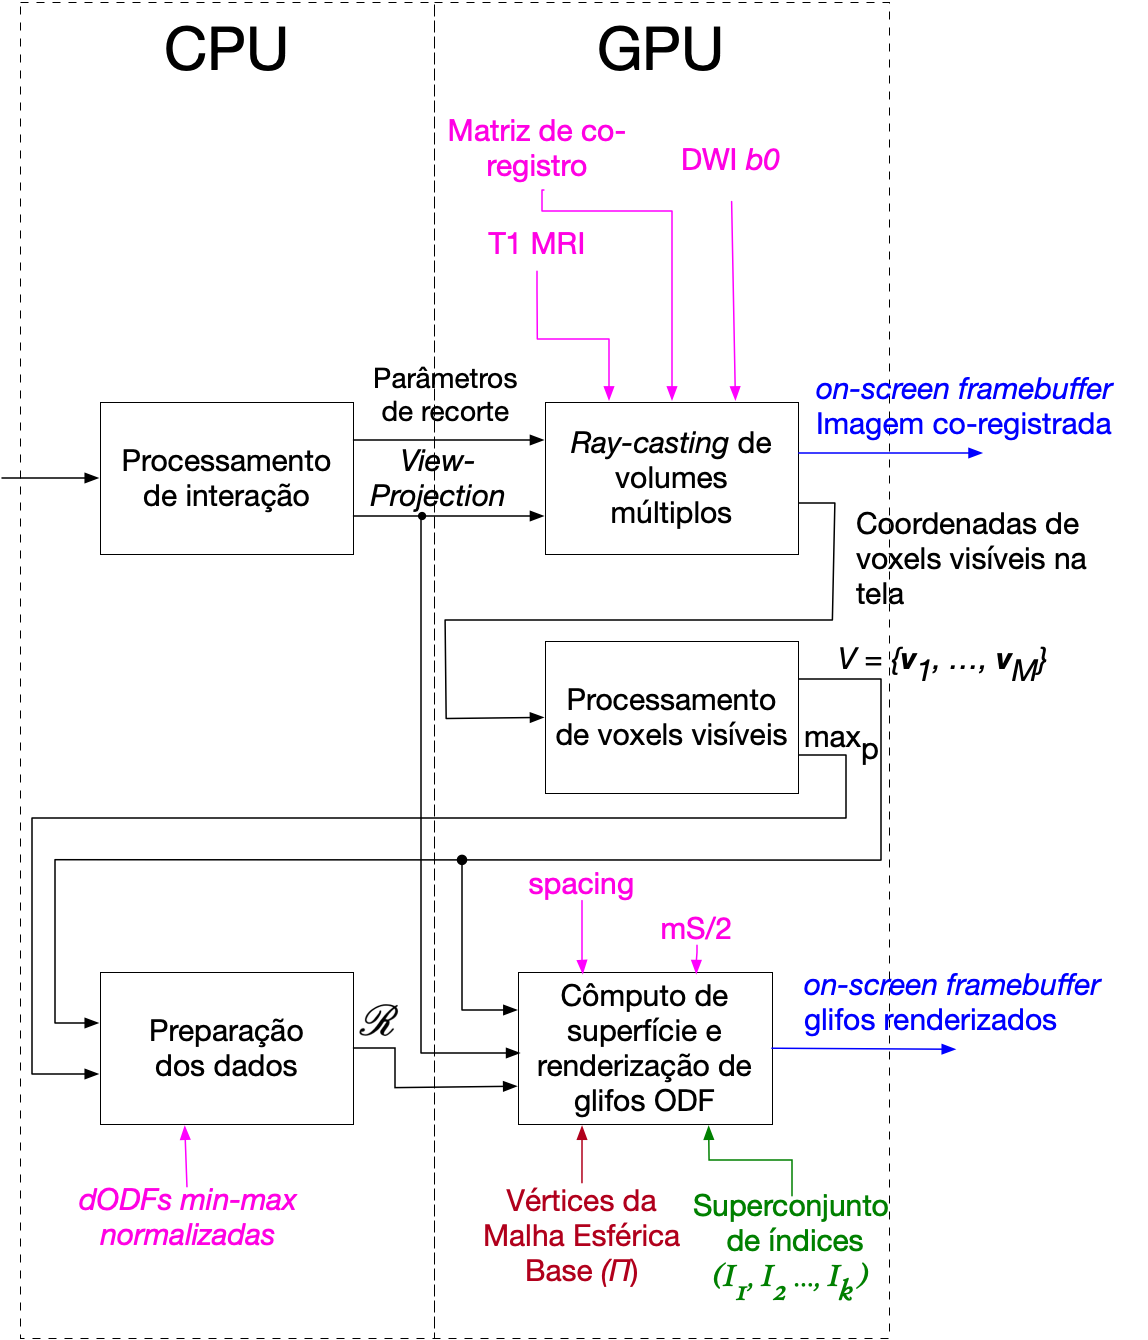
\includegraphics[width=.7\linewidth, angle=0]{figs/Esquema_Glifo/fluxograma_glifos_VMTK.png}
    \caption{
    Renderização multimodal para glifos ODF. A cor azul representa a saída a ser desenhada, armazenada no \textit{framebuffer} (FB); a cor magenta se refere a dados pré-computados. Os estágios de \textit{raycasting} do volume e processamento de \textit{voxels} visíveis estão descritos por \citeonline{voltoline2021}. O estágio de preparação dos dados de ODF e renderização de glifos ODF estão descritos na Seção \ref{sec::renderizacao_de_glifos_ODF}.
    }
    \label{fig::vmtk_simplified}
\end{figure}

\textcolor{magenta}{
Nossa solução para minimizar a transferência de dados consiste em explorar a resolução da percepção visual, o uso de renderização por instâncias, exploração da simetria de ODFs e o uso de memória de textura. Na Subseção \ref{ssec::geometria_base}, descrevemos a geometria base que é deformado por cada conjunto de amostras de ODF. Na Subseção \ref{ssec::atributos}, descrevemos o leiaute de atributos que otimiza o uso de memória da GPU e o seu acesso.
}

%\subsection{Geometria base}
\subsection{Configuração simétrica}
\label{ssec::geometria_base}

%\subsubsection{Considerações iniciais}

As ODFs são amostradas a partir dos vetores normais dos pontos de uma malha base esférica $(\Pi, I)$, onde $\Pi = [P_1, P_2, \dots, P_N]$ consiste num conjunto de pontos não repetidos e o conjunto $I$ são os índices que referenciam os pontos de $\Pi$ para formar os triângulos que sintetizam a malha. Estabelecemos duas condições para a estrutura de dados, nas quais tiramos proveito da simetria de dados das ODFs e para que façamos a malha ser adaptativa para parâmetros de visualização. Estas condições tem impacto direto no tráfego de dados CPU-GPU, conforme discutido na Subseção \ref{ssec::atributos}.

A primeira condição, conforme já discutido no capítulo \ref{chapter::metodos_hardi} na forma de armazenamento de dados da ODF tira vantagem da simetria e armazena os pontos em metade de uma esfera. Propomos que os pontos simétricos em relação aos eixos coordenados de $\Pi$ estejam dispostos de forma consecutiva na memória, i. e. $P_{2i+2} = -P_{2i+1}$, $(0 \leq i \leq \frac{N-2}{2})$, o que nos leva a uma estrutura de dados $\Pi = [P_1, -P_1, P_3, -P_3, \dots, P_{N-3}, -P_{N-3}, P_{N-1}, -P_{N-1}]$.

A segunda condição objetiva fazer a geometria base do glifo ser adaptativa como uma sub-malha da malha esférica base. Seja $k$ o número de sub-malhas de $(\Pi, I)$, onde cada sub-malha é denotada por $(\Pi_i, I_i)$,  $(0 \leq i < k)$, adicionalmente, o número de pontos das sub-malhas é crescente de acordo com os sub-índices, i.e. se $(0 \leq i < j < k)$, implica $|\Pi_j| > |\Pi_i|$. Sugerimos que cada sub-malha $(\Pi_i, I_i)$ seja simétrica em relação a origem e os primeiros $|\Pi_i|$ elementos na estrutura de dados de $\Pi$ corresponda aos elementos de $\Pi_i$. Note que esta condição também implica que, para $i$, $j$ tais $0 \leq i < j < k$, $\Pi_i$ é subconjunto de $\Pi_j$.

\subsection{Indexação dos pontos}
%\subsubsection{Formulação da geometria e estruturação de dados}
\label{sssec::formulação_da_geometria_e_estruturação_de_dados}

\todo[inline]{O procedimento de subdivisão não ficaria melhor no Cap. 2 quando se apresenta diferentes alternativas de subdivisões? Este procedimento entra como subdivisões uniformes}
\textcolor{magenta}{
Conforme mencionado no capítulo \ref{chapter::metodos_hardi}, escolhemos o conjunto de malhas derivada da $2^k$-ésima ordem de tesselação do icosaedro. O algoritmo para obtermos a tesselação de $2^k$-ésima ordem é um processo iterativo repetido $k$ vezes que se inicia com o icosaedro. Cada triângulo da malha é subdividido em quatro em cada iteração, onde os novos novos vértices adicionados são computados pela projeção da mediana dos pares de pontos conectados por uma aresta na esfera. Assim, o conjunto de vértices da $2^k$-ésima ordem contém todos os vértices das iterações anteriores. Adicionalmente, são todos simétricos com relação a origem. O processo de subdivisão de um triângulo está ilustrado na Fig. \ref{fig::triangle_icosahedron} e o algoritmo para se obter esta categoria de malha pode ser encontrado em \citeonline{luna2012}. Adicionalmente, a Fig. \ref{fig::icosphere} do Capítulo \ref{chapter::metodos_hardi} ilustra malhas esféricas desta categoria.
}

\textcolor{magenta}{
\begin{figure}[htb]
    \centering
    %\rule{6cm}{3cm}
    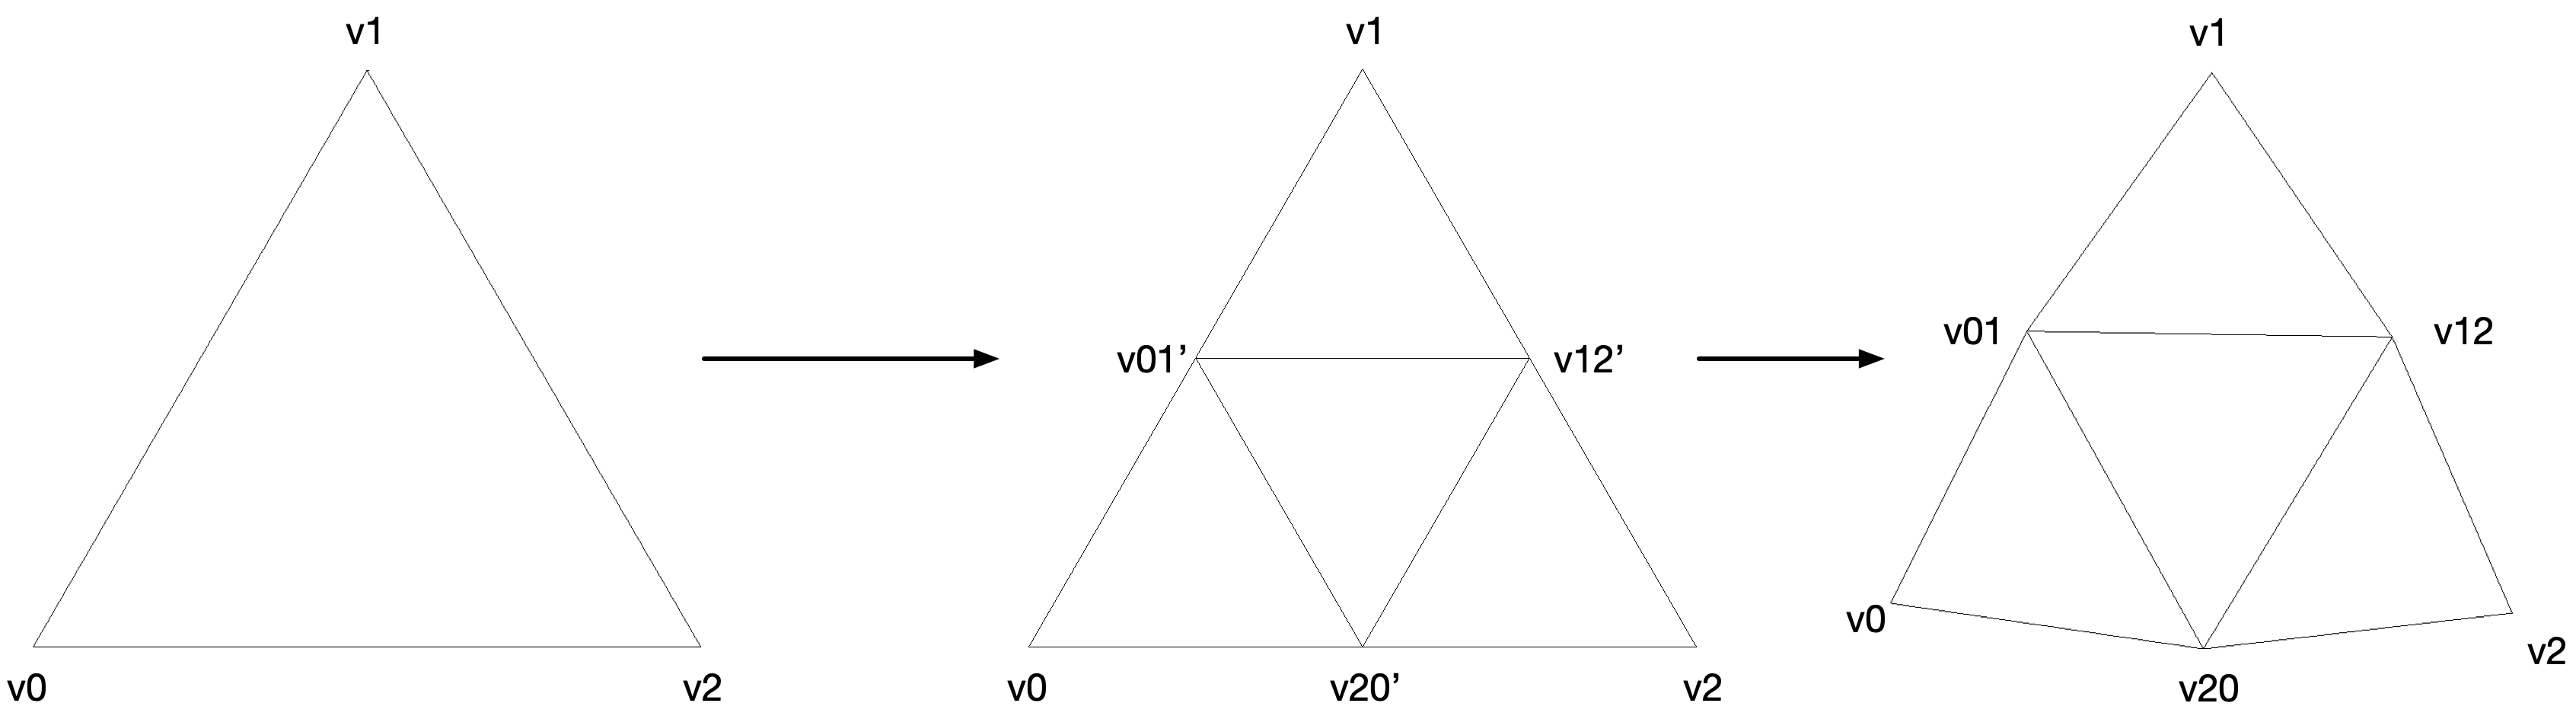
\includegraphics[width=1.0\linewidth, angle=0]{figs/Esquema_Glifo/ico_subdivision.png}
    \caption{
    Subdivisão de um triângulo para formar quatro na formação da malha esférica a partir da tesselação de $2^k$-ésima ordem a partir da partir da $2^{k-1}$-ésima. O triangulo formado pelos vértices $v0$, $v1$ e $v2$ é subdividido em quatro, onde as medianas  $v01'$, $v12'$ e $v20'$ são computadas e suas respectivas projeções na esfera $v01$, $v12$ e $v20$ são adicionados ao conjunto de vértices.
    }
    \label{fig::triangle_icosahedron}
\end{figure}
}

Há dois problemas adicionais que precisamos enfrentar no que diz respeito a obtenção de malhas esféricas através da subdivisão do icosaedro. O primeiro é garantir que os vértices simétricos estejam de forma consecutiva na memória e o segundo diz respeito a que não haja repetição de pontos em $\Pi$. O algoritmo para subdivisão do icosaedro em \citeonline{luna2012} insere vértices repetidos, pois há diversos pares de pontos conectados que definem mais de um triângulo.

A nossa abordagem para resolver esse problema consiste em identificar e deletar pontos replicados para termos somente uma amostra de cada em $\Pi$ e, após isso, ordenar o conjunto de dados $\Pi$ para que os simétricos estejam de forma consecutiva na memória, e essa mudança de estrutura de dados tem que ser compensada no conjunto de índices $I$. Para resolver estes problemas, propomos dois algoritmos que resolvem essas questões de forma genérica que são executados após cada iteração da subdivisão do icosaedro. O Algoritmo \ref{alg::tira_redundancia_pontos} certifica que os pontos redundantes são removidos, e o Algoritmo \ref{alg::reordena_simetricos} certifica que os pontos simétricos estarão em sequência na memória.

\begin{algorithm}
\caption{Algoritmo para retirada de pontos repetidos em estrutura de dados de vértices}
\label{alg::tira_redundancia_pontos}
\begin{algorithmic}[1]
\Procedure{ShrinkVertexSet}{$\Pi$, $I$}
 \State $I' \gets \{0, 1, 2, ..., |\Pi| - 1\}$
\State $i \gets 0$
\While{$i < |\Pi| - 1$} \label{alg::svs_pt1_inicio}
    \State $j \gets i + 1$
    \While{$j < |\Pi|$}
        \If {$\Pi[i] = \Pi[j]$}
            \State $I'[j] \gets i$
        \EndIf
        \State $j \gets j + 1$
    \EndWhile
    \State $i \gets i + 1$
\EndWhile \label{alg::svs_pt1_fim}
\State $\Pi_{size} \gets |\Pi|$
\State $i \gets 0$
\While{$i < \Pi_{size} - 1$} \label{alg::svs_pt2_inicio}
    \State $j \gets i + 1$
    \While{$j < \Pi_{size}$}
        \If{$\Pi[i] = \Pi[j]$}
            \State DELETE $\Pi[j]$ \label{alg::delete}
            \ForEach{$c \in I'$ \textbf{and} $c > j$}
                \State $c \gets c - 1$
            \EndFor
            \State $j \gets j - 1$
            \State $\Pi_{size} \gets \Pi_{size} - 1$
        \EndIf
        \State $j \gets j + 1$
    \EndWhile
    \State $i \gets i + 1$
\EndWhile \label{alg::svs_pt2_fim}
\ForEach{$c \in I$} \label{alg::resetI}
    \State $c \gets I'[c]$
\EndFor
\EndProcedure
\end{algorithmic}
\end{algorithm}

 \begin{algorithm}
 \caption{Pseudocódigo que sequencia vértices simétricos na memória}
 \label{alg::reordena_simetricos}
 \begin{algorithmic}[1]
 \Procedure{AlignSymmetricalMesh}{$\Pi$, $I$}
 \State $I' \gets \{0, 1, 2, ..., |\Pi| - 1\}$
 \State $i \gets 0$
 \While{$i < |\Pi| - 1$} 
     \State $j \gets i + 1$
     \While{$j < |\Pi|$}
         \If {$\Pi[i] = -\Pi[j]$}
             \State Swap($\Pi[i+1]$, $\Pi[j]$) \label{alg::troca}
             \ForEach{$c \in I$} \label{alg::compensacao_inicio}
                \If{$c = i+1$}
                    \State $c \gets j$
                    \State CONTINUE
                \ElsIf{$c = j$}
                    \State $c \gets i+1$
                    \State CONTINUE
                \EndIf
             \EndFor
             \State \textbf{break}
         \EndIf 
         \State $j \gets j + 1$
         \If {$j = |\Pi|$}
            \State \textbf{return} ERROR\_MESH\_NOT\_SYMMETRICAL
         \EndIf
     \EndWhile \label{alg::compensacao_fim}
     \State $i \gets i + 2$
\EndWhile
 \EndProcedure
 \end{algorithmic}
 \end{algorithm}
 
 O Algoritmo \ref{alg::tira_redundancia_pontos} pode ser dividido em duas partes e tem no vetor $I'$ o seu ponto crucial de funcionamento. Cada $I'[i]$ armazena está associado ao $i$-ésimo elemento de $\Pi$. Após a deleção dos elementos repetidos em $\Pi$, $I[i]$ guarda o índice do ponto que é igual a $\Pi[i]$ antes da deleção dos vértices repetidos.
 
 A primeira parte do algoritmo (Linhas \ref{alg::svs_pt1_inicio} até \ref{alg::svs_pt1_fim}) consiste trocar os vértices repetidos apontados por $I'$ para a sua primeira ocorrência em $\Pi$, visto que as demais ocorrências irão ser apagadas. A segunda parte do algoritmo (Linhas \ref{alg::svs_pt2_inicio} até \ref{alg::svs_pt2_fim}) consiste na deleção dos vértices repetidos, o comando DELETE na linha \ref{alg::delete} considera que a o processo de deleção do elemento consiste em deslocar os seus elementos conseguintes na memória para o endereço anterior\footnote{O funcionamento descrito é similar à função std::erase aplicada a classe std::vector em C++}, consequentemente, isto é compensado no conjunto de índices $I'$ pelo decremento de todos os índices apontados com valores maiores do que $j$. Na linha \ref{alg::resetI}, o elementos no conjunto de índices $I$ são corrigidos para referenciar para nova versão sem redundância de $\Pi$.
 
O Algoritmo \ref{alg::reordena_simetricos}, consiste na detecção dos simétricos e a troca de posição de pontos em índices ímpares para os simétricos dos índices pares em $\Pi$ (Linha \ref{alg::troca}) na posição anterior e a compensação no conjunto de índices $I$ (Linhas \ref{alg::compensacao_inicio} até \ref{alg::compensacao_fim}).

\subsection{Multi-resolução}

Sendo assim, o Algoritmo \ref{alg::setIcosahedroBase} mostra os procedimentos para subdivisão do icosaedro, bem como onde os algoritmos \ref{alg::tira_redundancia_pontos} e \ref{alg::reordena_simetricos} se situam. A variável $k$ representa a quantidade de iterações, $\mathbf{I}$ é o superconjunto que contém os conjuntos de índices para diferentes resoluções do glifo e $\Pi$ a lista de vértices do icosaedro tesselado de ordem $2^k$.

Nas linhas \ref{alg::subdivide_icosahedron} e \ref{alg::project_onto_sphere}, temos o algoritmo de subdivisão dos triângulos em quatro e sua projeção na esfera \cite{luna2012}, obtidos como ilustrado na Fig. \ref{fig::triangle_icosahedron}, adicionalmente, os novos vértices gerados são alocados após o fim da estrutura de dados dos vértices base, o que faz com que, os vértices do icosaedro estejam situados no início da estrutura, seguidos dos vértices gerados pela primeira subdivisão, depois dos vértices gerados na segunda subdivisão e assim sucessivamente.

 \begin{algorithm}
 \caption{Pseudocódigo que gera diferentes esferas a partir de tesselações de ordem $2^k$ do icosaedro.}
 \label{alg::setIcosahedroBase}
 \begin{algorithmic}[1]
 \Function{SetIcosahedronSet}{$k$}
 \State $\mathbf{I} = \{I_0, I_1, ..., I_{k-1}, I\}$
 \State $(\Pi, I) = \text{(Icosahedron.Vertices, Icosahedron.Indices)}$  \cite{luna2012} \label{alg::init_icosahedron}
 \State $i \gets 0$
 \While{$i < k$}
    \State ShrinkVertexSet($\Pi, I$)
    \State AlignSymmetricalMesh($\Pi, I$)
    \State $I_i \gets I$
    \State ($\Pi$, $I$) = Subdivide($\Pi, I$) \cite{luna2012}  \label{alg::subdivide_icosahedron}
    \State ($\Pi$) = ProjectOntoSphere($\Pi$) \cite{luna2012} \label{alg::project_onto_sphere}
    \State $i \gets i + 1$
\EndWhile
    \State \textbf{return} $(\Pi, \mathbf{I})$
 \EndFunction
 \end{algorithmic}
 \end{algorithm}
 

Assim, definindo $(\Pi, I)$ para ser a $2^{k}$-ésima ordem de tesselação para ser a malha esférica base e mantendo cada conjunto de índices de menor ordem a cada iteração, temos um conjunto de $k$ sub-malhas $(\Pi_0, I_0), (\Pi_1, I_1), ..., (\Pi_{k-1}, I_{k-1})$ definidos como as tesselações de $1^{a}$, $2^{a}$, ... $2^{k-1}$-ésima ordem. As Eq. \ref{eq::2ordem_icosphere_vertices}\footnote{Note que esta equação é a Eq. \ref{eq::icosa_samples} adaptada para $2^k$-ésima ordem de tesselação do icosaedro} e \ref{eq::2ordem_icosphere_triangulos} computam a quantidade de vértices e triângulos para esta categoria de malha em função da tesselação de ordem $2^k$, respectivamente.

\begin{equation}
\label{eq::2ordem_icosphere_vertices}
V = 10\times 4^k + 2
\end{equation}

\begin{equation}
\label{eq::2ordem_icosphere_triangulos}
\tau = 20\times 4^k
\end{equation}

Assim como mencionado no capítulo \ref{chapter::metodos_hardi}, por questões de memória, recomendamos k = 3, ou no máximo 4. Assim, formulamos a estrutura de dados que satisfaz as duas condições que estabelecemos a princípio, e é tal que os primeiros 12 elementos correspondem aos vértices do icosaedro, os 42 primeiros elementos correspondem aos vértices da $2^a$ ordem de tesselação, os 162 primeiros elementos correspondem a $4^a$ ordem de tesselação, os primeiros 642 elementos correspondam a $8^{a}$ ordem de tesselação, e, adicionalmente, os pontos simétricos são agrupados em sequencia na memória.

A estrutura de dados $\Pi$, e $I$, além dos índices que triangulam todas as sub-malhas, contidos ao superconjunto $\mathbf{I}$ no Algoritmo \ref{alg::setIcosahedroBase}, são enviados à GPU uma vez. Uma vez que os dados estão na GPU, e visando eficiência no processamento, sem comprometer a qualidade visual, escolhemos adaptativamente a geometria base entre estas malhas por um procedimento heurístico computado em tempo de execução baseado em $max_p$.

\section{Tráfego CPU-GPU}

\subsection{Escolha automática da geometria base}
\label{sssec::escolha_automatica_da_geometria_base}

A escolha da geometria base é baseada no \textit{trade-off} de \citeonline{voltoline2021}, que indica a quantidade mínima de triângulos para dado um $max_p$, que é dado por $\tau \geq 8\sqrt{max_p}$  ($max_p > 0$). Este \textit{trade-off} estabelece a quantidade mínima de triângulos a ser utilizada na malha que não sacrifica a qualidade de imagem dos glifos. Derivamos uma expressão para a escolha da sub-malha da malha esférica base a partir do caso de igualdade do \textit{trade-off}, no qual substituímos a quantidade de triângulos como uma função da ordem de tesselação do icosaedro e mapeamos o icosaedro para o caso $max_p = 0$. A expressão base está na Eq. \ref{eq::icosa_order_base}:

\begin{equation}
\label{eq::icosa_order_base}
     20\times 4^k - 20\times 4^0 = 8\sqrt{max_p}
\end{equation}

Derivamos $t$ ($t \leq k$) na Eq. \ref{eq::icosa_order} como a ordem de tesselação do icosaedro escolhida. Como $t$ é inteiro positivo, para satisfazer o \textit{trade-off} de \citeonline{voltoline2021}, arrendondamos o valor para cima.

\begin{equation}
\label{eq::icosa_order}
     t = \lceil \frac{1}{2}\log_2{(\frac{2}{5}\sqrt{max_p} + 1)} \rceil
\end{equation}

Para geometria base derivada da $2^t$-ésima ordem de tesselação, devemos ser atentos a dois procedimentos na seleção da malha em tempo de execução. O primeiro consiste na ativação do seu respectivo conjunto de índices para triangulação. O segundo consiste em setar a quantidade de dados de ODF por glifo enviado à GPU como uma função de sua quantidade de vértices, o que será discutido mais a frente, na Subseção \ref{ssec::atributos}.

\subsection{Instanciação}

\section{Processamento em GPU}

\subsubsection{Fator de escala para geometria}

Finalmente, sugerimos escalar a a malha base pelo fator de escala $mS$ para proporcionar a máxima ocupância em tela, fazendo o glifo, cuja ODF está contida no intervalo $[0, 1]$, caber no seu respectivo \textit{voxel}:

\begin{equation}
\label{eq:spacings}
mS = min(spacing_x, spacing_y, spacing_z)
\end{equation}


onde $spacing_x$, $spacing_y$, $spacing_z$ é o espaço entre duas amostras adjacentes nos eixos x, y e z, respectivamente.





%The vertices and amount of triangles and the expression for the vertices and triangles number for each $2^k$ tessellation are in Table \ref{tab::icosahedron_set}. In practice, we recommend $k$ to be equal to 3 or 4, at most. Values of above those may incur a prohibitive amount of memory for pre-computed ODF samples in a DWI.



\section{Glifos ODF}
\label{sec::glifos_odf}

%Como descrito na seção \ref{sec::trabalhos_relacionados_glifos}
\subsection{Superfície}

A superfície do glifo da ODF no voxel de coordenadas $\mathbf{r}$ $\psi(\mathbf{r}, \mathbf{\hat{u}})$ consiste na plotagem polar esférica onde $R(\mathbf{\hat{u}}) = \psi(\mathbf{r}, \mathbf{\hat{u}})$. A plotagem polar esférica $R(\mathbf{\hat{u}})$ é uma superfície na qual a distância da origem para um dos seus respectivos pontos na direção $\mathbf{\hat{u}}$ é dado por $R(\mathbf{\hat{u}})$.

% é dada por  na modulação do raio na direção $\mathbf{u}$ de uma esférica de acordo com uma versão normalizada do seu valor de imagem na função $\psi(\mathbf{u})$. A normalização que fizemos neste trabalho para representação está representado na equação \ref{eq::normglifo2}.

%\begin{equation}
%\label{eq::normglifo2}
%    R(\mathbf{u}) = \frac{\psi(\mathbf{u}) - min(\psi(\mathbf{u}))}{max(\psi(\mathbf{u})) - min(\psi(\mathbf{u}))}
%\end{equation}
\subsection{Cor}

As componentes r, g e b do mapeamento de cor esférica do glifo é dado em função da direção $\mathbf{\hat{u}} = (u_x, u_y, u_z)$, como definido em Eq. \ref{eq::cor_glifo} e ilustrado nos glifos da Fig. \ref{fig::glifo_ilustrado}. Esta forma de mapear, além de simples, é comumente utilizado pela comunidade DWI. %\todo{É imprescincível adicionar esta informação?}\sout{Não foi implementado o cômputo de vetores normais à superfície representadas pelo glifo, que consequentemente não tem iluminação associada.}

\begin{equation}
\label{eq::cor_glifo}
    r = |u_x| ~~~~ g = |u_y| ~~~~ b = |u_z|, 
\end{equation}

\begin{figure}[ht]

%\subfigcapskip = -5pt
    \centering
    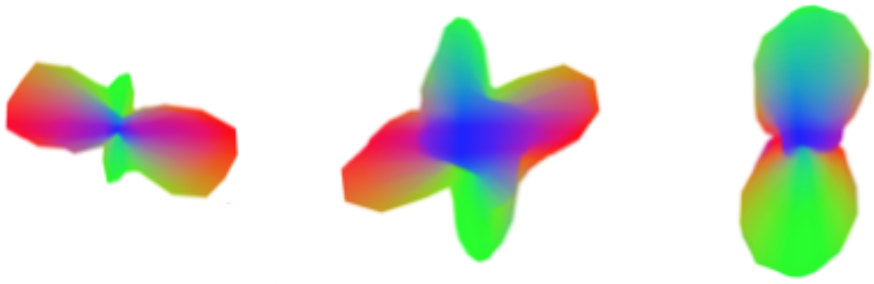
\includegraphics[width=.8\linewidth, angle=0]{figs/Esquema_Glifo/Glifos3Ex.png}
    \caption{Exemplos de glifos ODF. Os glifos consistem em uma superfície plotagem polar com a cor esquematizada de acordo com a equação \ref{eq::cor_glifo}.}
    \label{fig::glifo_ilustrado}
   \hspace{1pt}
\end{figure}

A respeito de planos anatômicos, a cor vermelha (r) representa a direção mediolateral, a verde (g), se refere a direção anteroposterior, e a azul (b), a direção inferior-superior.



\section{Renderização multimodal de glifos superquádricas}
\label{sec::superquadricas}

\citeonline{voltoline2021} propuseram um algoritmo de renderização multimodal de glifos superquádricos sobre o seu respectivo MRI anatômico ponderado em T1. O volume $b0$, seu respectivo MRI T1 e a matriz rígida que co-registra ambos os volumes \cite{ting2014} são enviadas à GPU.

O algoritmo de renderização é dividido em três estágios: (1) renderização do DWI e do volume anatômico; (2) detecção dos \textit{voxels} visíveis e estimativa da cobertura máxima da projeção dos glifos em \textit{pixels}, para estimativa da resolução da malha; (3) renderização de \textit{voxels} visíveis na resolução estimada.

Para manter a compatibilidade do algoritmo com o Mac OSX, cuja versão máxima suportada do OpenGL é 4.1, eles desdobraram o algoritmo para estimação de cobertura máxima de \textit{pixels} para os glifos de um passo, onde a implementação é feita no \textit{compute shader} em um algoritmo de quatro passos, envolvendo \textit{vertex, geometry} e \textit{fragment shaders} baseados em rasterização. Para evitar transferência de dados entre CPU e GPU entre passos, o \textit{transform feedback buffer} foi aplicado. Adicionalmente, eles mostraram a utilização do mecanismo de \textit{additive blending} para obtenção do número máximo de \textit{pixels} ($max_p$), no qual o \textit{voxel} é projetado em um volume \textit{ray-casted}. Baseado em $max_p$, eles estabelecem uma heurística para estimação da resolução da malha.

Através de $max_p$, um \textit{tessellation shader} é acionado para gerar o \textit{skeleton} base dos superquádricos, no qual eles utilizam o comando renderização indireta por instâncias para desenhá-los com uma chamada desenho. Provendo a parâmetros particulares a cada \textit{voxel} que definem cada superquádrico, em cada instância o \textit{skeleton} é customizado para gerar o glifo e é posicionado em seu respectivo \textit{voxel} no espaço do volume.





\subsection{Atributos}
\label{ssec::atributos}



Para renderizarmos $M$ glifos com um comando de desenho, usamos instanciação de GPU. A geometria base selecionada, referente a $2^t$-ésima ordem de tesselagem do icosaedro é instanciada por um vetor de translação e amostras de ODF.

\subsubsection{Posicionamento}

Para $M$ \textit{voxels} visíveis, enviamos os vetores de translação como um atributo por instância, que é computado em função das coordenadas de \textit{voxel} $V(v_x, v_y, v_z)$ como:

\begin{align}
 \label{eq::translation}
    dx = (v_x + 0.5).spacing_x \nonumber\\
    dy = (v_y + 0.5).spacing_y \\
    dz = (v_z + 0.5).spacing_z \nonumber
\end{align}

Note que os dados de voxel visíveis retornados pelo algoritmo é armazenado em um buffer na GPU. Este dado é utilizado diretamente no algoritmo de renderização no \textit{vertex shader} para cômputo do atributo de translação.

\subsubsection{Dados de ODF}
\label{sssec::dados_de_odf}

Como mencionado no capítulo \ref{chapter::metodos_hardi}, aproveitamos a simetria dos dados de ODF para organizarmos os dados no domínio de um hemisfério. Para o voxel de coordenadas índice $\mathbf{r}$, os elementos são organizados como $\boldsymbol{\psi}(\mathbf{r}) = [
\psi(\mathbf{r}, \mathbf{n}_1),
\psi(\mathbf{r}, \mathbf{n}_3), ...,
\psi(\mathbf{r}, \mathbf{n}_{N-3}),
\psi(\mathbf{r}, \mathbf{n}_{N-1})]^T$. Onde cada elemento na K-ésima posição $\psi(\mathbf{r}, \mathbf{n}_{2K-1})$ desloca os pontos $P_{2K-1}$ e seu simétrico $P_{2K}$ na geometria base instanciada. Note que no capítulo \ref{chapter::metodos_hardi}, o armazenamento de amostras em um metade de uma esfera tem o objetivo de economia de memória, enquanto neste capítulo, tem o objetivo de minimizar o tráfego de dados CPU-GPU.

Para a geometria base escolhida, geramos uma matriz com os dados de ODF enviados à GPU como a matriz $\mathbf{R}_{\frac{V}{2}xM}$ (Eq. \ref{eq::R}), onde $V$ é o numero de vértices da geometria base, dado por $10 \times 4^t + 2$ (Eq. \ref{eq::2ordem_icosphere_vertices}). A $j$-ésima coluna consiste nos primeiros $V/2$ elementos de $\boldsymbol{\psi}(\mathbf{d_j})$. $\mathbf{R}$ é enviado à GPU como uma textura 2D de formato RGBA.

\begin{equation}
\label{eq::R}
\mathbf{R} = 
\begingroup % keep the change local
\setlength\arraycolsep{2pt}
\begin{bmatrix} 
    \psi(\mathbf{d}_{1}, \mathbf{n}_1) &
    \psi(\mathbf{d}_{2}, \mathbf{n}_1) & \cdots & 
    \psi(\mathbf{d}_{M}, \mathbf{n}_1)  \\
    
    \psi(\mathbf{d}_{1}, \mathbf{n}_3) &
    \psi(\mathbf{d}_{2}, \mathbf{n}_3) & \cdots & 
    \psi(\mathbf{d}_{M}, \mathbf{n}_{3}) \\ \vdots & \vdots & \vdots & \vdots  \\
    
    \psi(\mathbf{d}_{1}, \mathbf{n}_{V-1}) & 
    \psi(\mathbf{d}_{2}, \mathbf{n}_{V-1}) & \cdots & 
    \psi(\mathbf{d}_{M}, \mathbf{n}_{V-1})
\end{bmatrix}.
\endgroup
\end{equation}

Cada \textit{texel} no formato RGBA suporta quatro valores. Agrupamos os valores escalares da j-ésima coluna $[
\psi(\mathbf{d}_{j}, \mathbf{n}_1),
\psi(\mathbf{d}_{j}, \mathbf{n}_3), ...,
\psi(\mathbf{d}_{j}, \mathbf{n}_{V-3}),
\psi(\mathbf{d}_{j}, \mathbf{n}_{V-1})
]^T$ de quatro em quatro, como mostrado na Fig. \ref{fig::texelfetch}. Consequentemente, em cada acesso de \textit{texel}, temos quatro valores escalares $
\psi(\mathbf{d}_{j}, \mathbf{\mathbf{n}_{8K+1}})$ (R), $
\psi(\mathbf{d}_{j}, \mathbf{\mathbf{n}_{8K+3}})$ (G), $
\psi(\mathbf{d}_{j}, \mathbf{\mathbf{n}_{8K+5}})$ (B), $
\psi(\mathbf{d}_{j}, \mathbf{\mathbf{n}_{8K+7}})$ (A). Nos quais deslocamos quatro pares de pontos simétricos na geometria base $P_{8K+1}$, $-P_{8K+1}$, $P_{8K+3}$, $-P_{8K+3}$, $P_{8K+5}$, $-P_{8K+5}$, $P_{8K+7}$, $-P_{8K+7}$ para o j-ésimo glifo visível (também j-ésima instância). Desta forma, as dimensões da textura com dados ODF é $ \frac{V/2}{4} \times M$. Se $\frac{V}{2}$ não é divisível por quatro, é necessário inserir mais linhas abaixo da última com valores \textit{dummy}, para que o número de linhas se torne divisível, o que certifica que cada coluna de $\mathbf{R}$ possa ser acessada com o índice de instância na GPU.

\begin{figure}[ht]
%\subfigcapskip = -5pt
    \centering
    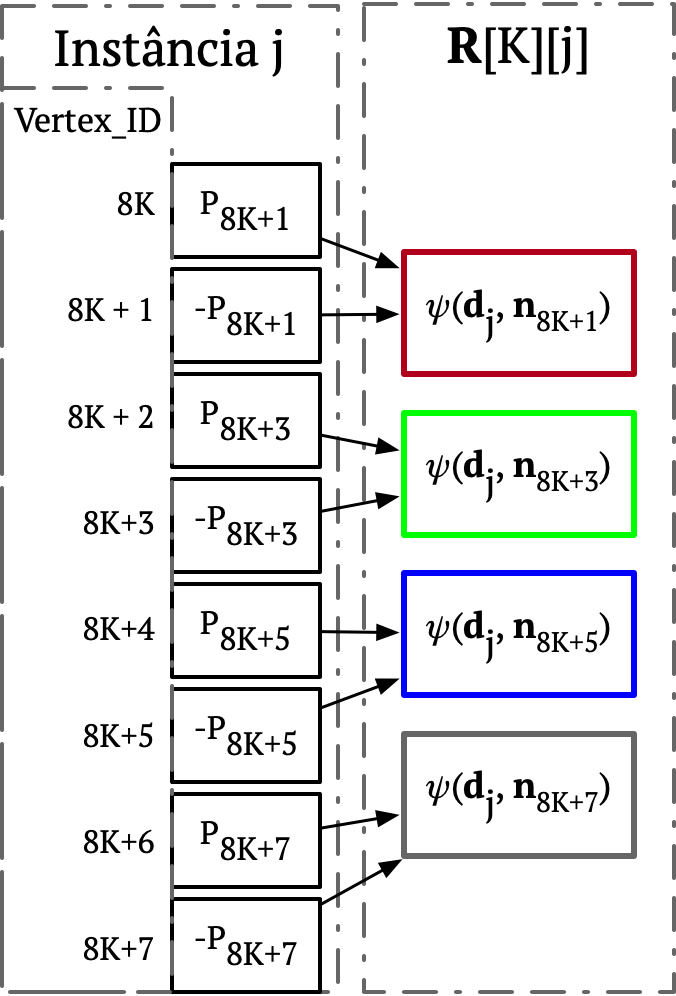
\includegraphics[width=.45\linewidth, angle=0]{figs/Esquema_Glifo/texellookup.png}
    \caption{Ilustração do acesso nas componentes RGBA em \textit{texel} na textura \textbf{R} no índice $K$ e $j$. O \textit{texel} é acessado pelas threads que processam os vertices de índices 8K, 8K+1, ..., 8K+7 em uma instância $j$. Os blocos de contorno vermelho, azul, verde e cinza ilustram as componentes R,G,B e A do \textit{texel}, respectivamente.}
    \label{fig::texelfetch}
   %\hspace{1pt}
\end{figure}

Os dados de ODF são acessados no \textit{vertex shader}, quando cada glifo da $j$-ésima instância é processada. Os \textit{texels} com índice de coluna $K = \lfloor\frac{Vertex\_ID}{8} \rfloor$ são acessados para deslocar oito pontos. Usamos a função \textit{texelFetch} para acessar diretamente a textura de ODF utilizando coordenadas não-normalizadas $(j, \lfloor\frac{Vertex\_ID}{8} \rfloor)$. O valor utilizado para \textit{lookup} da componente  para deslocar o seu respectivo ponto na geometria base no \textit{vertex shader} é acessível pela análise do resto da divisão por oito do Vertex\_ID, como ilustrado na Fig. \ref{fig::texelfetch}. Adicionalmente, utilizando a notação via colchetes, onde as componentes R, G, B e A são mapeados nos índices 0, 1, 2 e 3, respectivamente, o escalar de ODF pode ser mapeado por $\lfloor (Vertex\_ID \mod{8})/2 \rfloor$\footnote{A função em OpenGL para \textit{lookup} em função dos índices de instância e vértice é dada por texelFetch($\mathbf{R}$,ivec2((gl\_VertexID)/8, gl\_InstanceID), 0)[(gl\_VertexID\%8)/2]}.

\subsection{Síntese}

Podemos sintetizar as transformações aplicadas a cada vértice $P_K$ em coordenadas homogêneas na $j$-ésima instância por uma multiplicação matricial no \textit{vertex shader} por uma matriz $G_{Kj}$. Esta matriz pode ser sintetizada da seguinte forma:

\begin{equation}
    G_{Kj} = \mathbf{M_{vp}}\cdot M_D \cdot M_S \cdot M_{Kj}
\end{equation}

onde $M_{kj}$ é a matriz que escalona o ponto $P_K$ na $j$-ésima instância por $\psi(\mathbf{d}_j, \mathbf{n}_k)$, $M_S$ se refere a transformação de escala, dado por Eq. \ref{eq:spacings}, $M_D$ é a matriz de translação do glifo, centrado na origem para o centro do seu respectivo \textit{voxel} no espaço do volume, dado pela Eq. \ref{eq::translation}, e, adicionalmente, $\mathbf{M_{vp}}$ é a matriz \textit{view-projection}, que configura parâmetros de visão e projeção.
